% !TeX spellcheck = fr_FR

% TODO: Replace scan images with clean text where possible

\documentclass[a4paper, 10pt]{report}

\usepackage[french]{babel}
\usepackage[T1]{fontenc}

\usepackage{amsmath, amssymb, amsfonts}

\usepackage{hyperref}
\usepackage{geometry}

\usepackage{xcolor}
\usepackage{graphicx}

\usepackage{fancyhdr}
\usepackage{lastpage}

\usepackage{enumitem}

\geometry{
	a4paper,
	left=25mm,
	right=25mm,
	top=35mm,
	bottom=25mm,
	headsep=5mm,
	headheight=20mm,
}

\definecolor{solution}{HTML}{E5E4E2}
\providecommand{\abs}[1]{\lvert#1\rvert}
\providecommand{\norm}[1]{\lVert#1\rVert}

\begin{document}
	
	\renewcommand{\headrule}{%
		\vspace{-4pt}\hrulefill
		\raisebox{-6.8pt}{\ 
\includegraphics[height=5mm]{../../icon.png}}
		\hrulefill
	}	
	\pagestyle{fancy}
	\fancyhf{}
	
	\fancyhead[L]{\small \slshape Automne 2024}
	\fancyhead[C]{\Large \bfseries Logique et Théorie des Ensembles\\
		Série 07-B}
	\fancyhead[R]{\small Buff Mathias}
	\fancyfoot[L]{
		\small Source files available at:
		\href{https://github.com/MathiasBuff/bsc-math}
		{github.com/MathiasBuff/bsc-math}
	}
	\fancyfoot[R]{
		\small Page \thepage
		\hspace{1pt} /
		\pageref*{LastPage}
	}
	
	
	\noindent
	\textbf{Exercice 1.} Calculer les applications réciproques des
	applications suivantes :
	\begin{itemize}
		\item $f : \begin{aligned}
			&[0, 2\pi) \times \mathbb{R}^*_+
			&&\to \mathbb{R}^2 \setminus\{0\}\\
			&(\theta, r) &&\mapsto (r \cos \theta, r \sin \theta)
		\end{aligned}$
		%
		\item $\chi : \begin{aligned}
			&\mathcal{P}(E)	&&\to \{0, 1\}^E\\
			&A &&\mapsto \chi_A
		\end{aligned}$
		%
		\item $g \circ f$ pour $f: E \to F$ et $g: F \to G$ bijectives
		(en fonction des réciproques de $f$ et $g$)
	\end{itemize}
	
	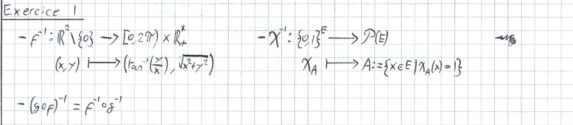
\includegraphics{ex01.jpg}
	
	\vspace{5mm}
	\noindent
	\textbf{Exercice 2.} Supposons qu'il existe une bijection entre
	$A$ et $B$, montrer qu'il existe une bijection entre
	$\mathcal{P}(A)$ et $\mathcal{P}(B)$.
	
	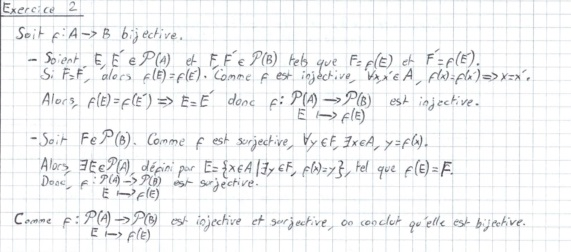
\includegraphics{ex02.jpg}	
	
	\newpage
	
	\fancyhf{}
	\renewcommand{\headrule}
	{\rule{\textwidth}{0pt}}
	\fancyfoot[R]{
		\small Page \thepage
		\hspace{1pt} /
		\pageref*{LastPage}
	}
	
	\noindent
	\textbf{Exercice 3.} Montrer que les relations suivantes sont des
	relations d'ordre.
	
	\begin{enumerate}[label=\arabic*.]
		\item L'ordre lexicographique sur $\mathbb{R}^2$ séfini par
		$(x, y)\mathcal{R}(a, b)$ ssi $x < a$ ou $x = a$ et $y \leq b$.
		
		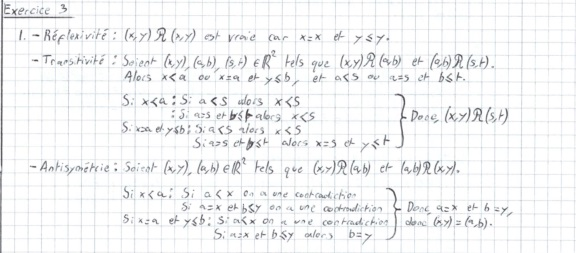
\includegraphics{ex03-p1.jpg}
		
		\item La divisibilité sur $\mathbb{N}$.
		
		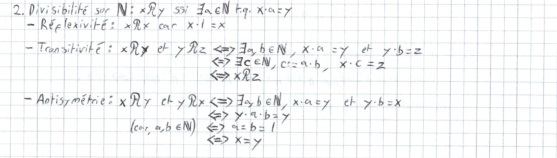
\includegraphics{ex03-p2.jpg}
		
		\item La relation $\mathcal{R}$ sur $\mathbb{N}^*$ définie par
		$p\mathcal{R}q$ s'il existe $k \in \mathbb{N}^*$ tel que $q = p^k$.
		
		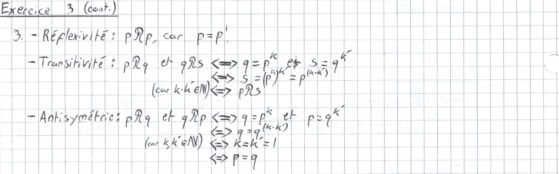
\includegraphics{ex03-p3.jpg}
		
		\item La relation $\mathcal{R}$ sur $(- \pi/2, \pi/2)$ définie par
		$x\mathcal{R}y$ si $\tan x \leq \tan y$.
		
		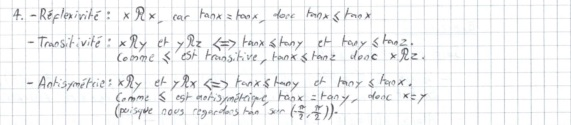
\includegraphics{ex03-p4.jpg}
	\end{enumerate}	
	
	\newpage
	
	\noindent
	\textbf{Exercice 4.} Existe-t-il une bijection de
	$(0,1)$ dans $[0,1]$ ?
	
	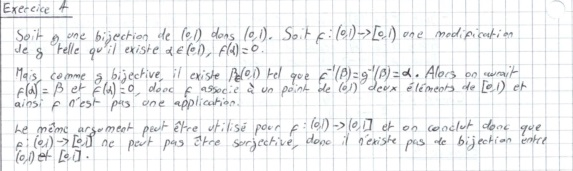
\includegraphics{ex04.jpg}
	
	\vspace{5mm}
	\noindent
	\textbf{Exercice 5.} (*Détails manquants dans la preuve du théorème
	de Cantor-Schröder-Bernstein).\\
	On utilise les notations de la preuve du théorème de
	Cantor-Schröder-Bernstein présentée en cours.
	\begin{enumerate}[label=\arabic*.]
		\item Montrer que $A \subset B$ implique $h(A) \subset h(B)$.
		\item Soit $f: E_1 \to F_1$ et $g: E_2 \to F_2$ avec
		$E_1 \cap E_2 = \emptyset$ et $F_1 \cap F_2 = \emptyset$.
		Montrer que si $f$ et $g$ sont bijectives, alors
		\[h: \begin{aligned}
			&E_1 \cup E_2 &\to \quad &F_1 \cup F_2\\
			&x &\mapsto \quad
				&\left\{\begin{aligned}
					&f(x) \text{ si } x \in E_1\\
					&g(x) \text{ si } x \in E_2\\
				\end{aligned}\right.
		\end{aligned}\]
		est bijective.
	\end{enumerate}
	
	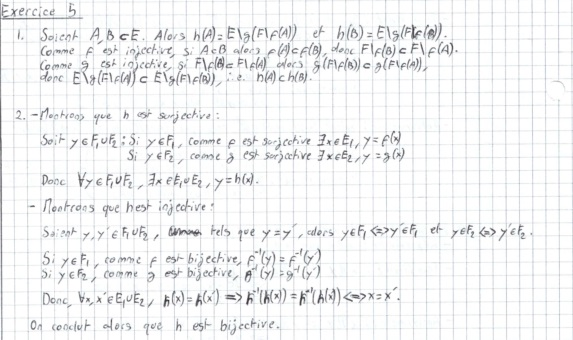
\includegraphics{ex05.jpg}
	
	
	
	
\end{document}
